\FloatBarrier
\section{Abbildungen}
\begin{figure}[!h]
	\caption{Systemmodell}
	\label{system_model:overview}
	\resizebox{\textwidth}{!} {
		\section{Systemmodelle}
\begin{figure}[!htb]
	\resizebox{\textwidth}{!} {
		\section{Systemmodelle}
\begin{figure}[!htb]
	\resizebox{\textwidth}{!} {
		\section{Systemmodelle}
\begin{figure}[!htb]
	\resizebox{\textwidth}{!} {
		\input{diagrams/system_model}
	}
\end{figure}
Das System basiert auf einer Client-Server-Architektur mit einer starken Trennung zwischen der Benutzerschnittstelle und dem Anwendungsserver. Der Nutzer gibt die benötigten Daten über die Benutzerschnittstelle ein. Die Verarbeitung findet serverseitig statt. Die \gls{Weboberflaeche} sendet hierfür eine Anfrage über einen \gls{Rest}-\gls{Webservice}
 und erhält über diese Schnittstelle eine Antwort zurück. \\
Auf dem Anwendungsserver werden die notwendigen Berechnungen durchgeführt, sowie die Produktdaten verarbeitet und gesichert.
	}
\end{figure}
Das System basiert auf einer Client-Server-Architektur mit einer starken Trennung zwischen der Benutzerschnittstelle und dem Anwendungsserver. Der Nutzer gibt die benötigten Daten über die Benutzerschnittstelle ein. Die Verarbeitung findet serverseitig statt. Die \gls{Weboberflaeche} sendet hierfür eine Anfrage über einen \gls{Rest}-\gls{Webservice}
 und erhält über diese Schnittstelle eine Antwort zurück. \\
Auf dem Anwendungsserver werden die notwendigen Berechnungen durchgeführt, sowie die Produktdaten verarbeitet und gesichert.
	}
\end{figure}
Das System basiert auf einer Client-Server-Architektur mit einer starken Trennung zwischen der Benutzerschnittstelle und dem Anwendungsserver. Der Nutzer gibt die benötigten Daten über die Benutzerschnittstelle ein. Die Verarbeitung findet serverseitig statt. Die \gls{Weboberflaeche} sendet hierfür eine Anfrage über einen \gls{Rest}-\gls{Webservice}
 und erhält über diese Schnittstelle eine Antwort zurück. \\
Auf dem Anwendungsserver werden die notwendigen Berechnungen durchgeführt, sowie die Produktdaten verarbeitet und gesichert.
	}
\end{figure}
\begin{figure}[!h]
	\caption{Loginseite des Systems mit Anmeldung über den \gls{Shibboleth Identity Provider} des \gls{KIT}}
	\label{fig:gui-login-1}
	\centering
	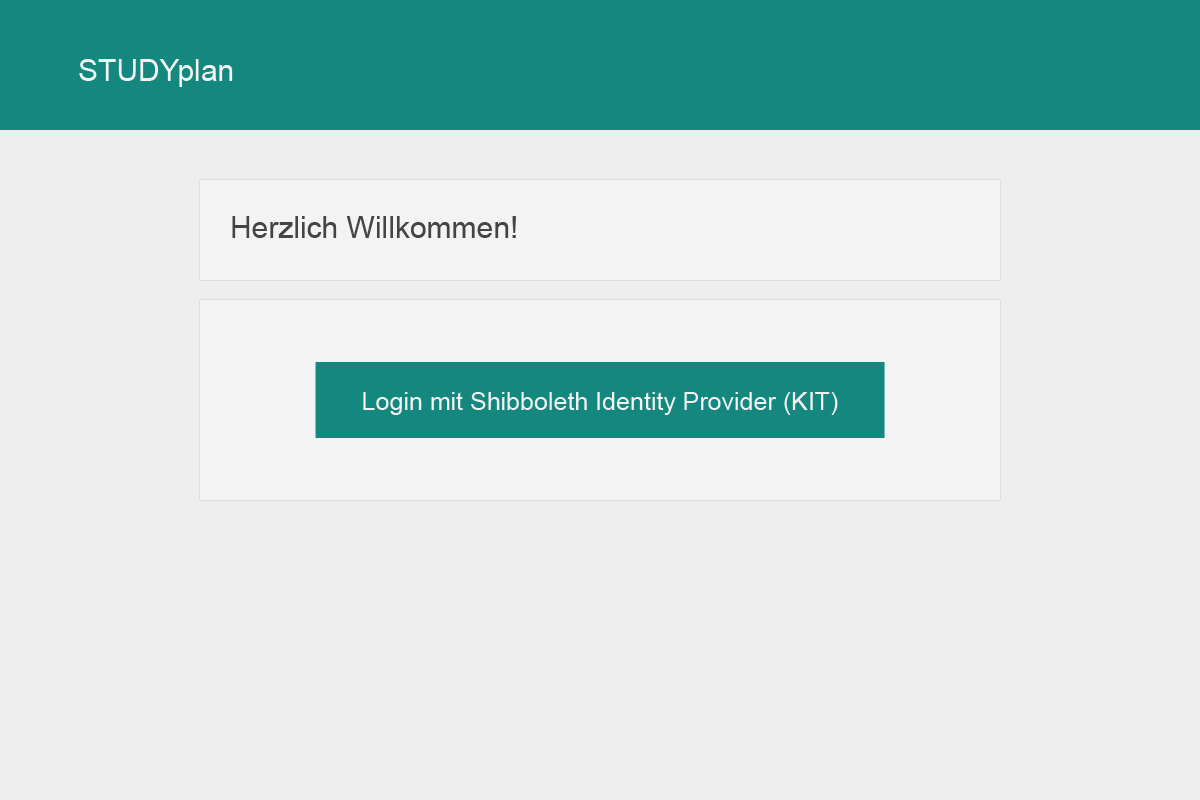
\includegraphics[width=0.8\textwidth]{../GUI/ergebnisse/login-1.png}
\end{figure}
\begin{figure}[!h]
	\caption{Erste Seite des Registrierungs"=\gls{Wizard}s mit Eingabe von Studienfach und Studienbeginn}
	\label{fig:gui-registrierung-1}
	\centering
	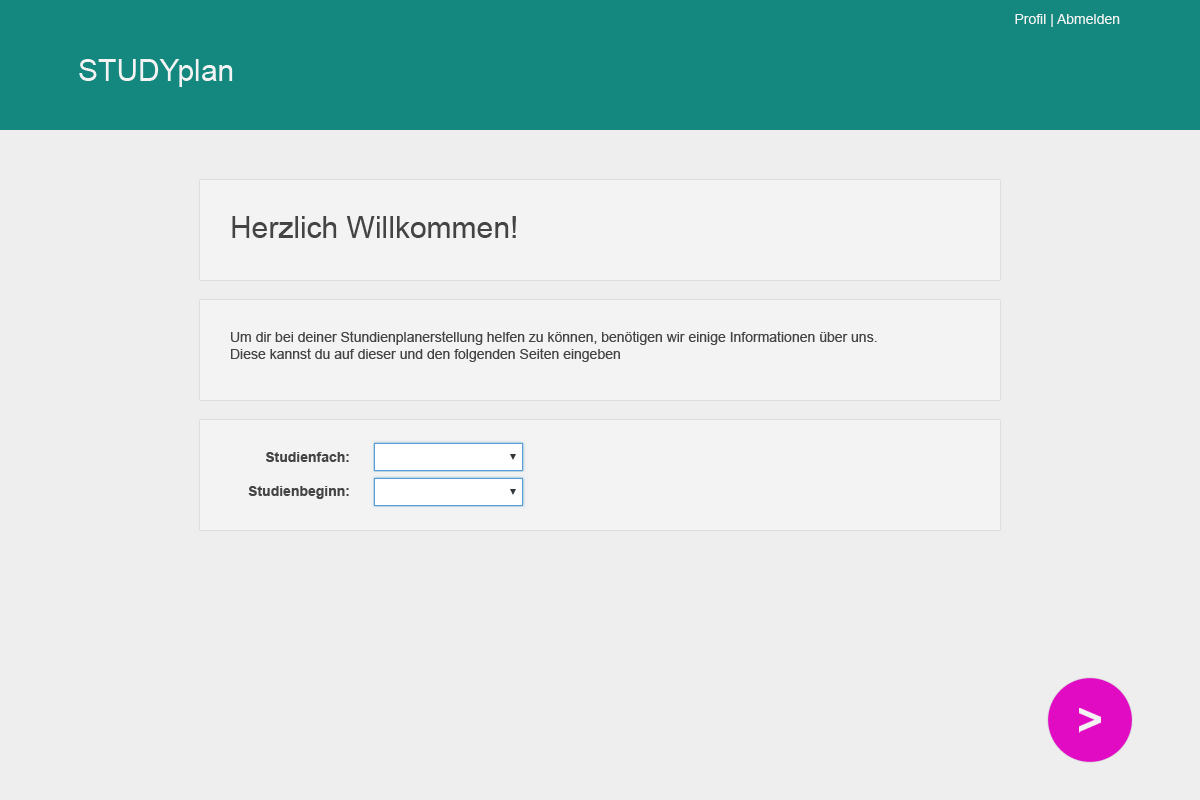
\includegraphics[width=0.8\textwidth]{../GUI/ergebnisse/registrierung-1.png}
\end{figure}

\begin{figure}
	\caption{Zweite Seite des Registrierungs"=\gls{Wizard}s mit Eingabe der schon begonnenen Module}
	\label{fig:gui-registrierung-2}
	\centering
	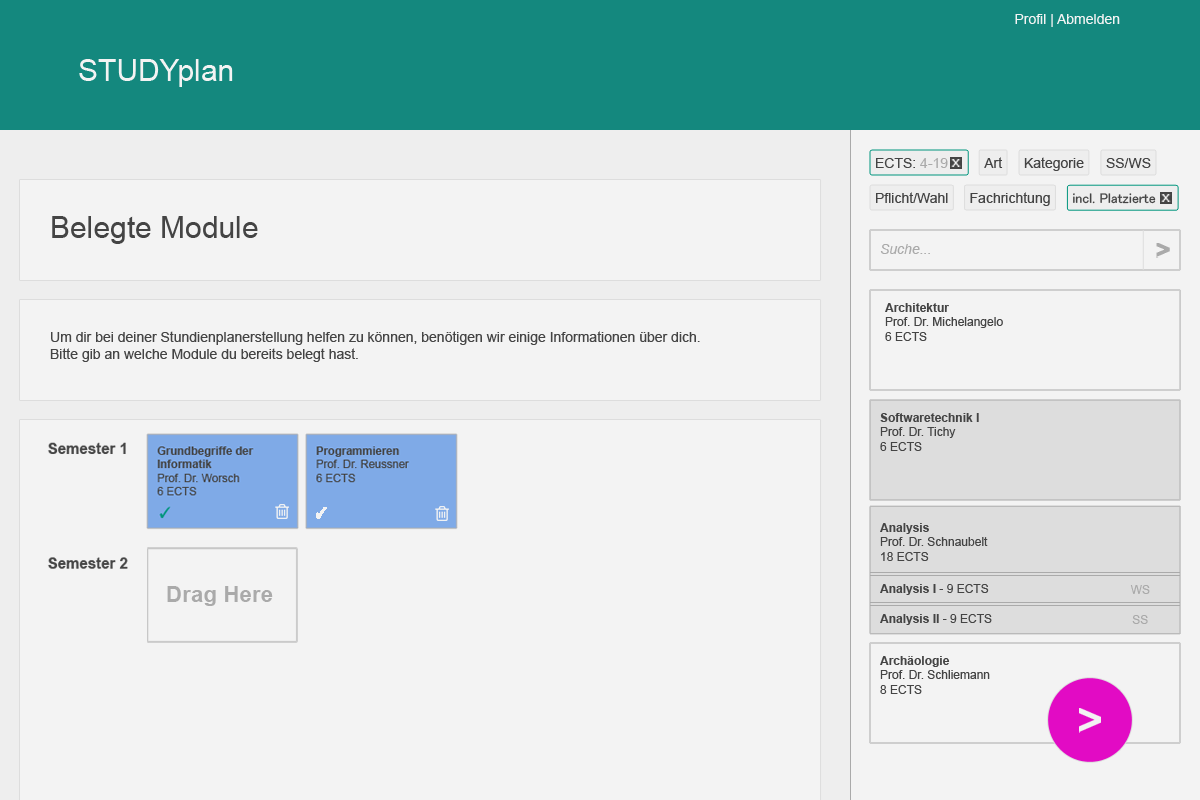
\includegraphics[width=0.9\textwidth]{../GUI/ergebnisse/registrierung-2.png}
\end{figure}

\begin{figure}
	\caption{Hauptseite des Systems}
	\label{fig:gui-hauptseite-1}
	\centering
	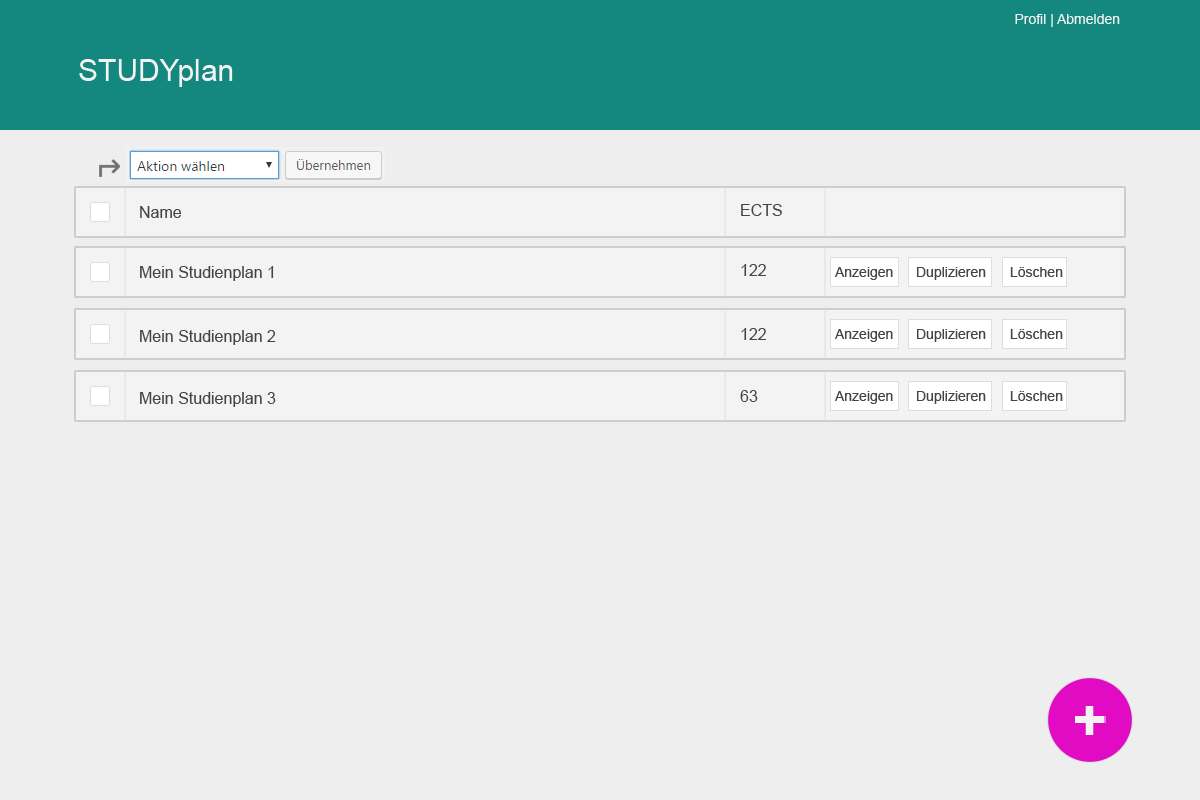
\includegraphics[width=0.9\textwidth]{../GUI/ergebnisse/hauptseite-1.png}
\end{figure}
\begin{figure}
	\caption{Manuelle Bearbeitung des Studienplans}
	\label{fig:gui-bearbeitung-1}
	\centering
	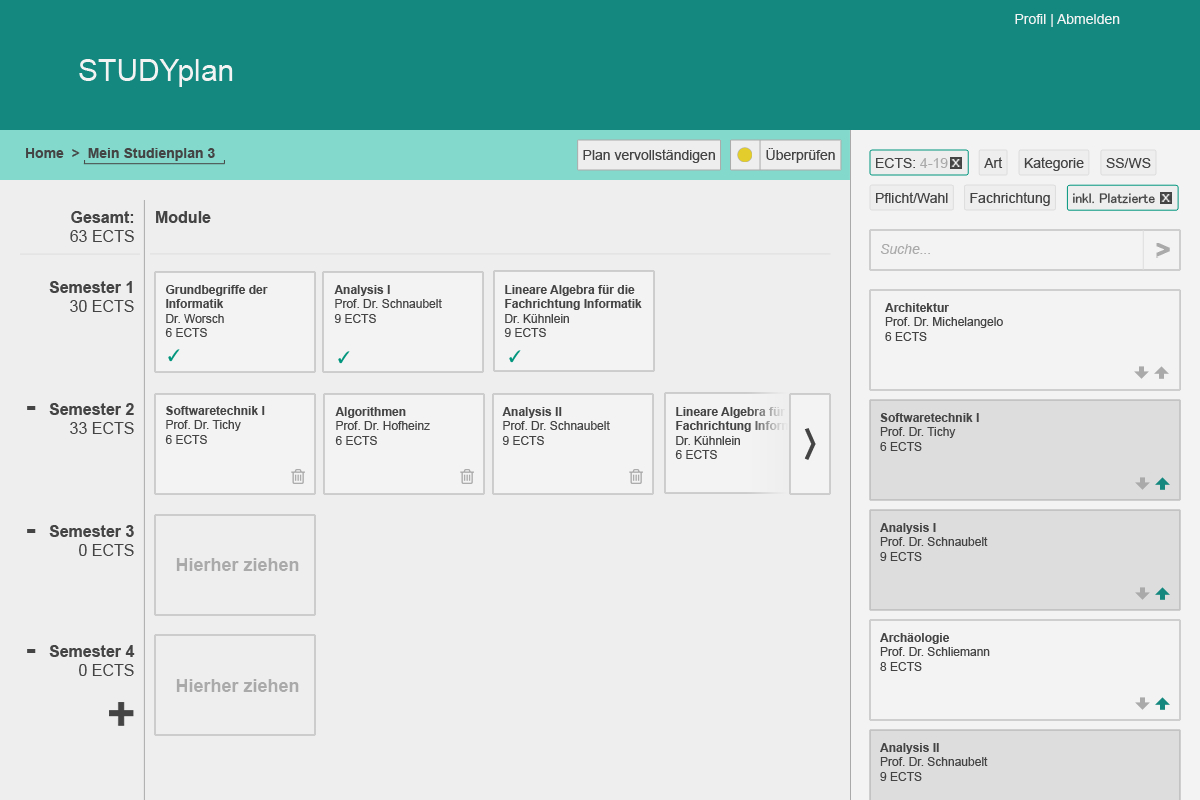
\includegraphics[width=0.9\textwidth]{../GUI/ergebnisse/bearbeitung-1.png}
\end{figure}
\begin{figure}
	\caption{Seitenleiste für Modulfilterung mit offener Kategorie-Auswahl}
	\label{fig:gui-module-filtern-1}
	\centering
	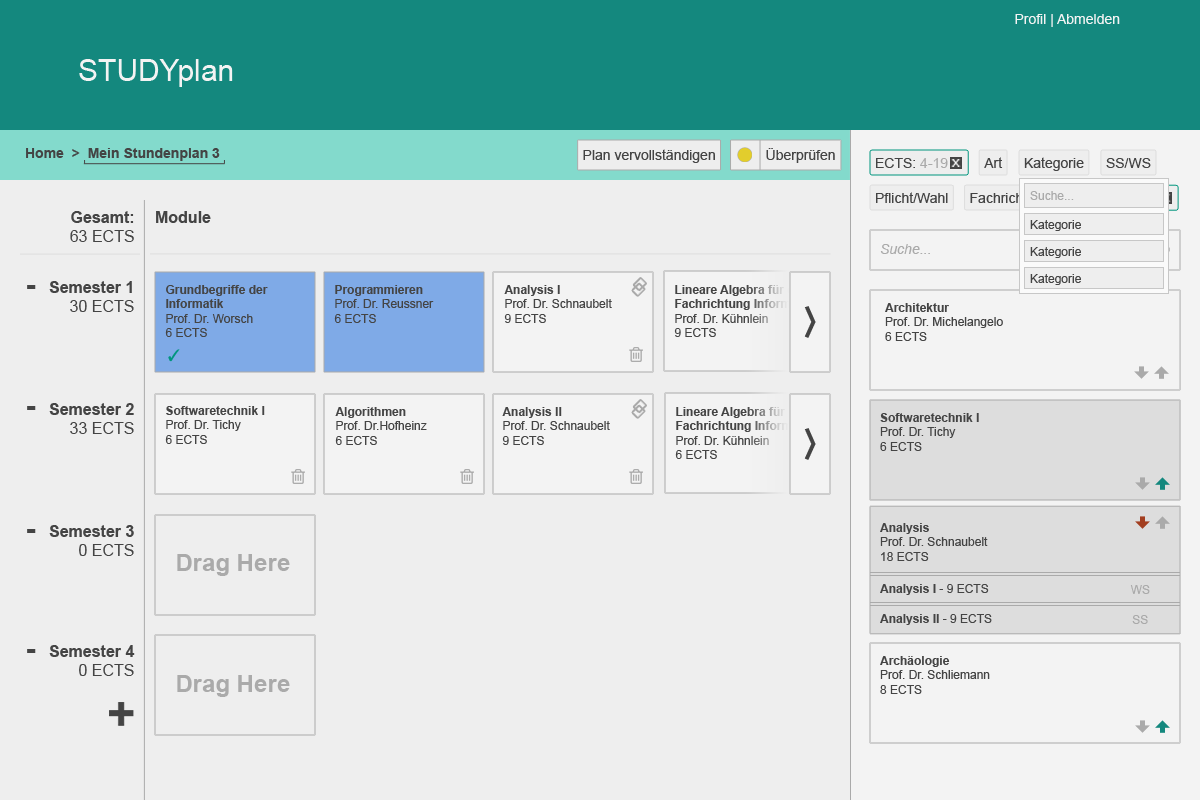
\includegraphics[width=0.9\textwidth]{../GUI/ergebnisse/module-filtern-1.png}
\end{figure}
\begin{figure}
	\caption{Seitenleiste für Modulfilterung mit offener ECTS-Auswahl}
	\label{fig:gui-module-filtern-2}
	\centering
	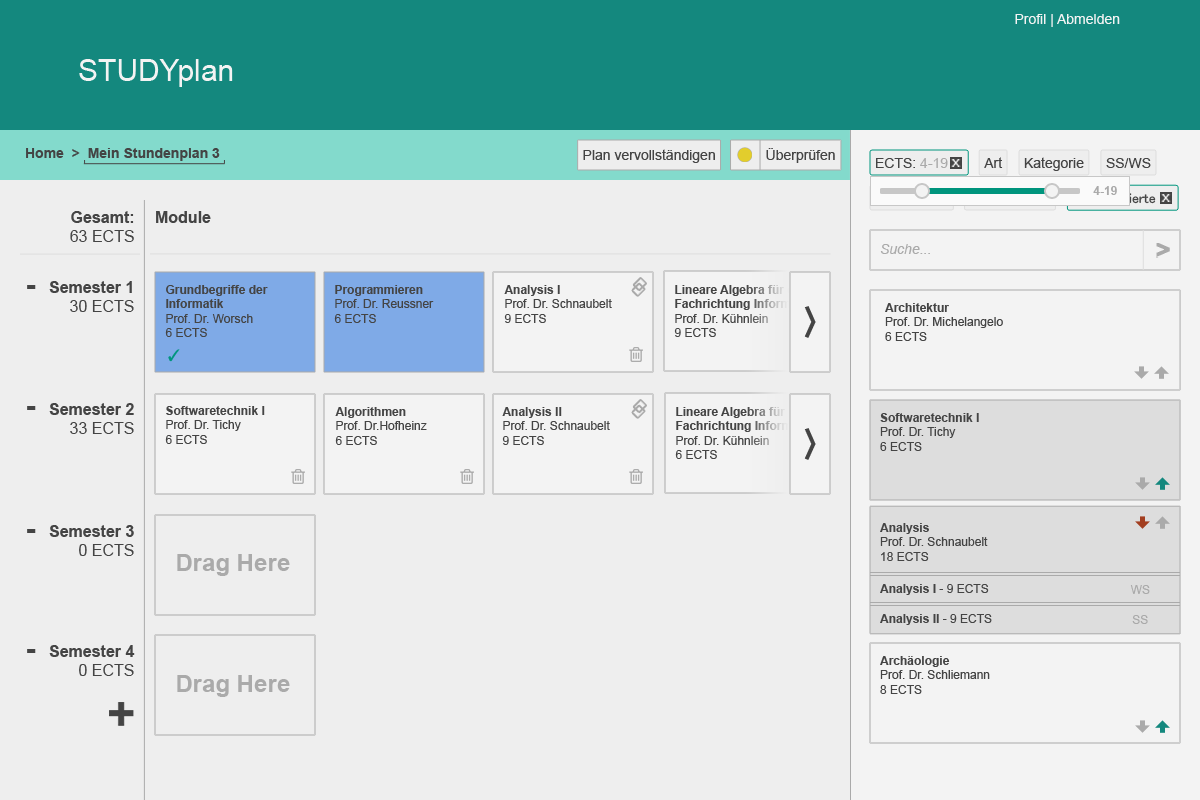
\includegraphics[width=0.9\textwidth]{../GUI/ergebnisse/module-filtern-2.png}
\end{figure}
\begin{figure}
	\caption{Detailansicht für Modul}
	\label{fig:gui-modul-info-1}
	\centering
	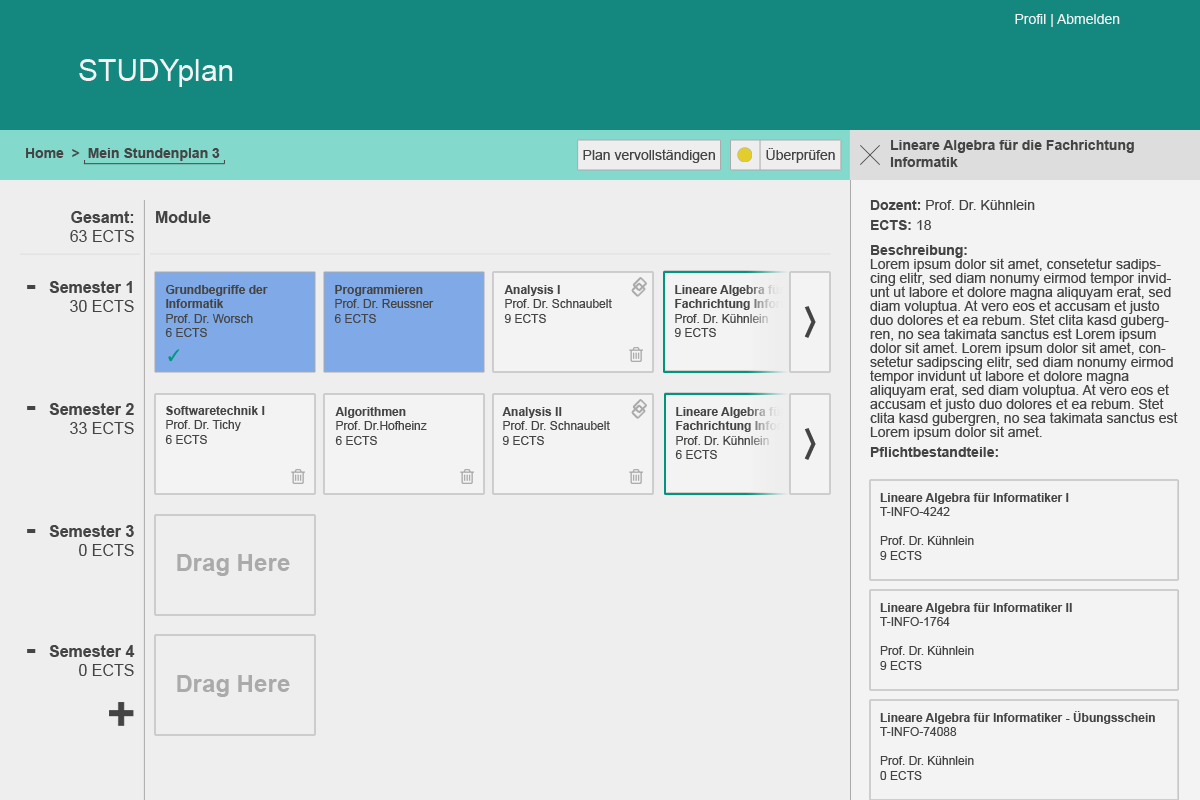
\includegraphics[width=0.9\textwidth]{../GUI/ergebnisse/modul-info-1.png}
\end{figure}
\begin{figure}
	\caption{1. Seite des Generierungs-Wizards}
	\label{fig:gui-generierung-1}
	\centering
	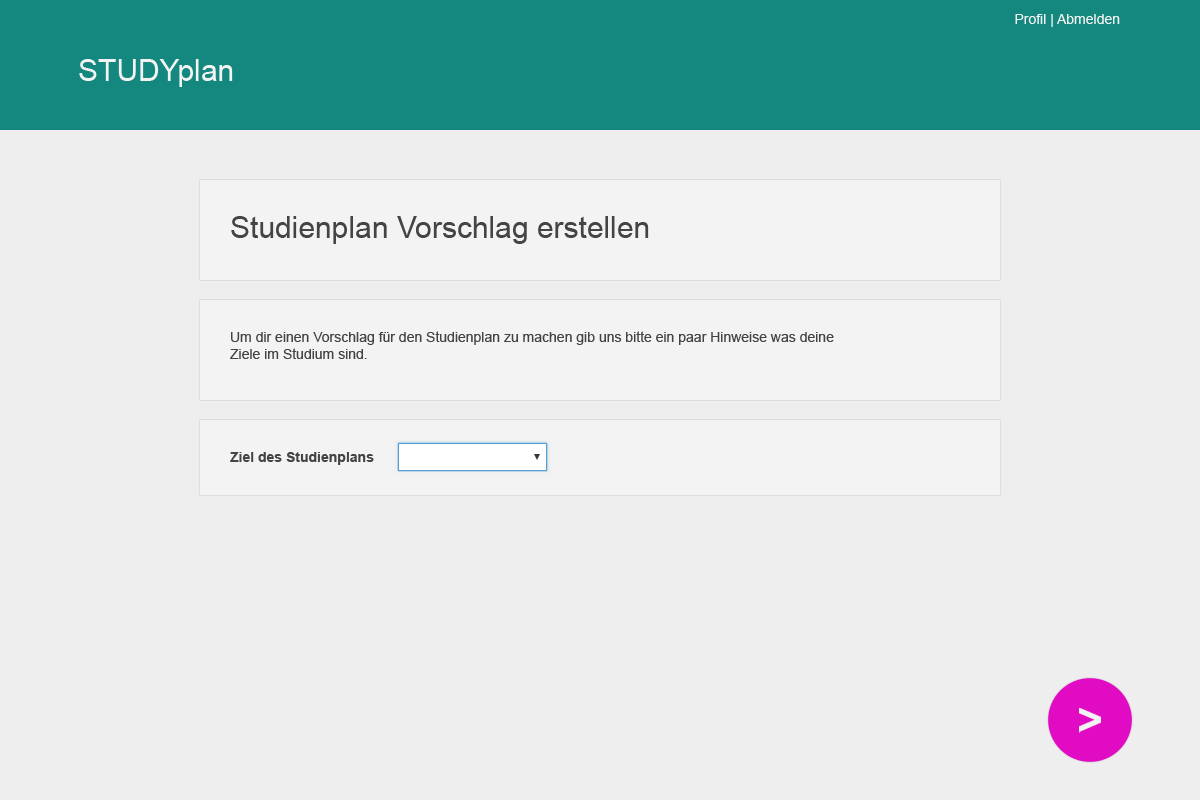
\includegraphics[width=0.9\textwidth]{../GUI/ergebnisse/generierung-1.png}
\end{figure}

\begin{figure}
	\caption{2. Seite des Generierungs-Wizard}
	\label{fig:gui-generierung-2}
	\centering
	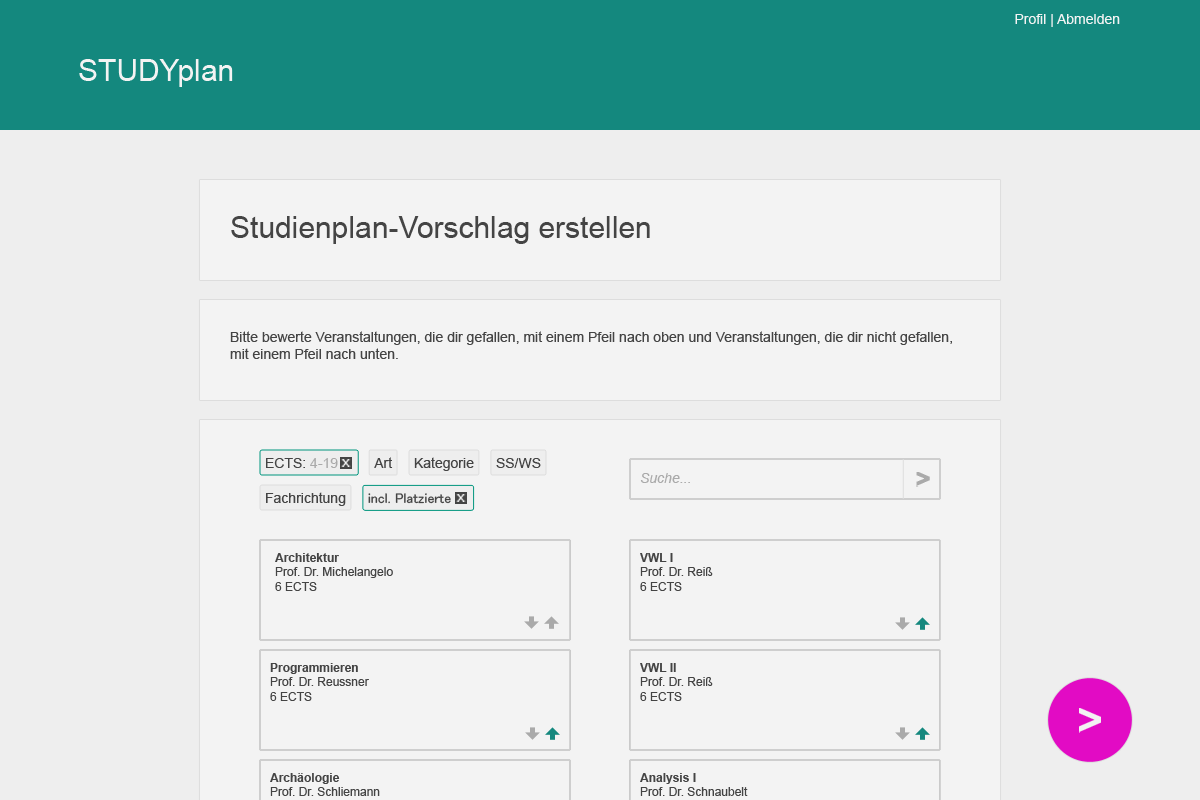
\includegraphics[width=0.9\textwidth]{../GUI/ergebnisse/generierung-2.png}
\end{figure}

\begin{figure}
	\caption{3. Seite des Generierungs-Wizard}
	\label{fig:gui-generierung-3}
	\centering
	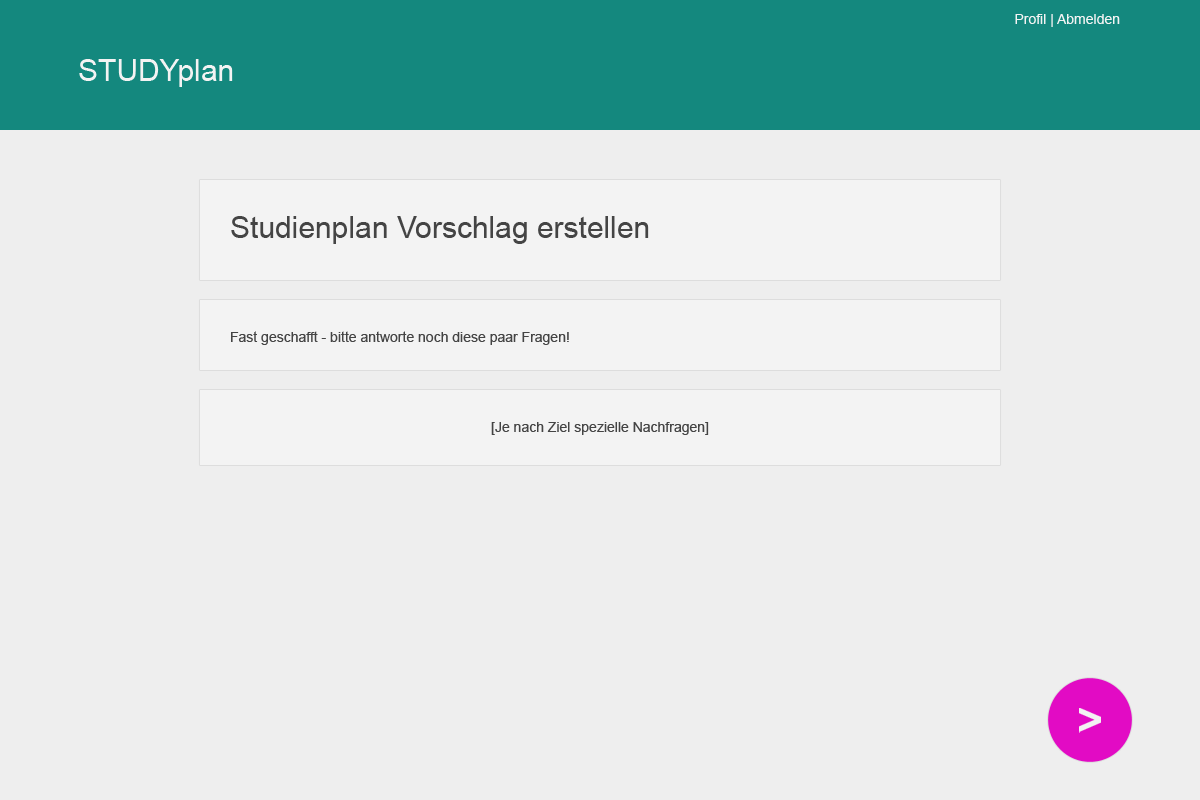
\includegraphics[width=0.9\textwidth]{../GUI/ergebnisse/generierung-3.png}
\end{figure}

\begin{figure}
	\caption{Anzeige des generierten Studienplans}
	\label{fig:gui-generierung-4}
	\centering
	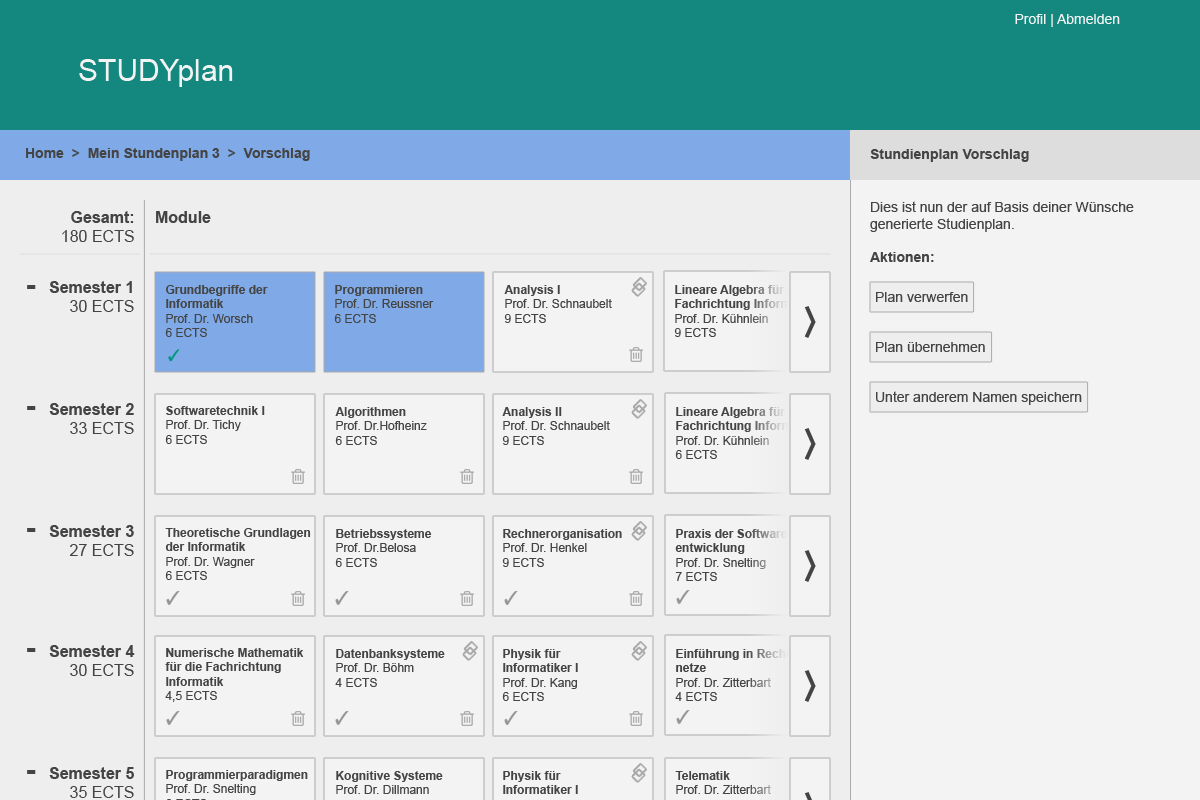
\includegraphics[width=0.9\textwidth]{../GUI/ergebnisse/generierung-4.png}
\end{figure}
\begin{figure}
	\caption{Erfolgreiche Verifizierung}
	\label{fig:gui-verifizierung-1}
	\centering
	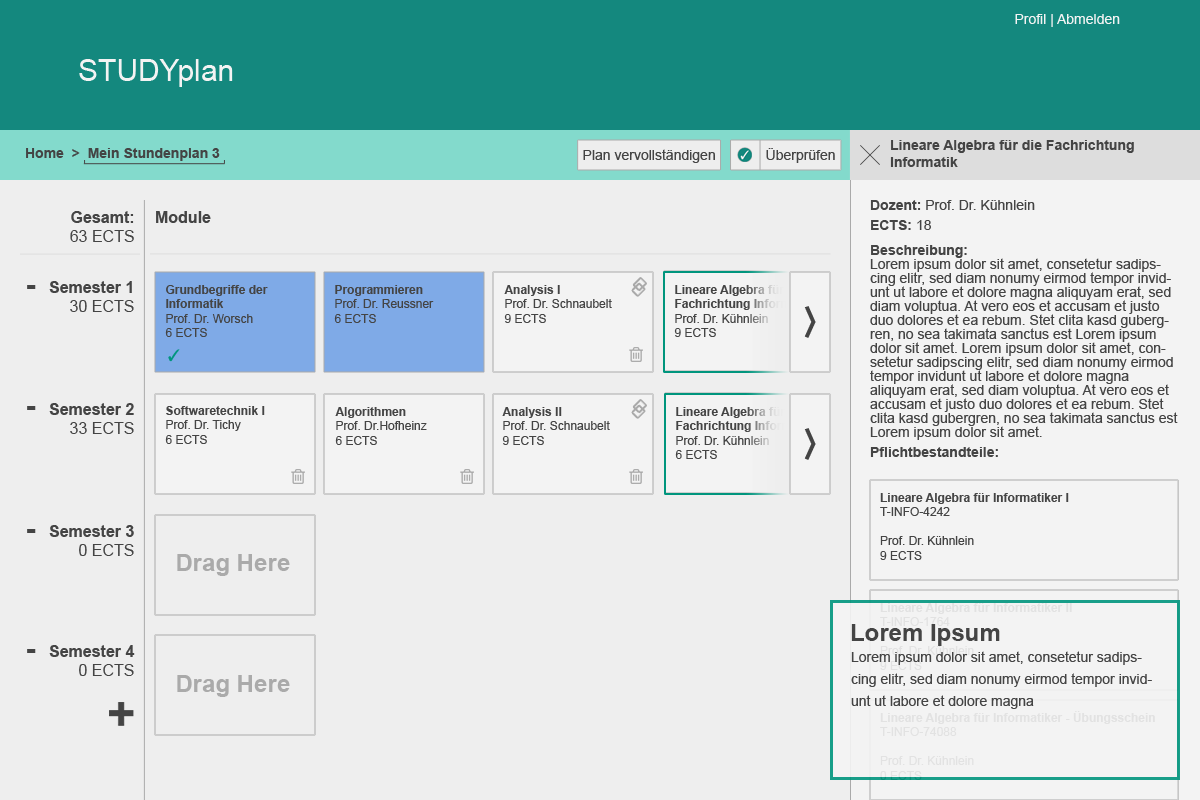
\includegraphics[width=0.9\textwidth]{../GUI/ergebnisse/verifizierung-1.png}
\end{figure}
\begin{figure}
	\caption{Fehlgeschlagene Verifizierung}
	\label{fig:gui-verifizierung-2}
	\centering
	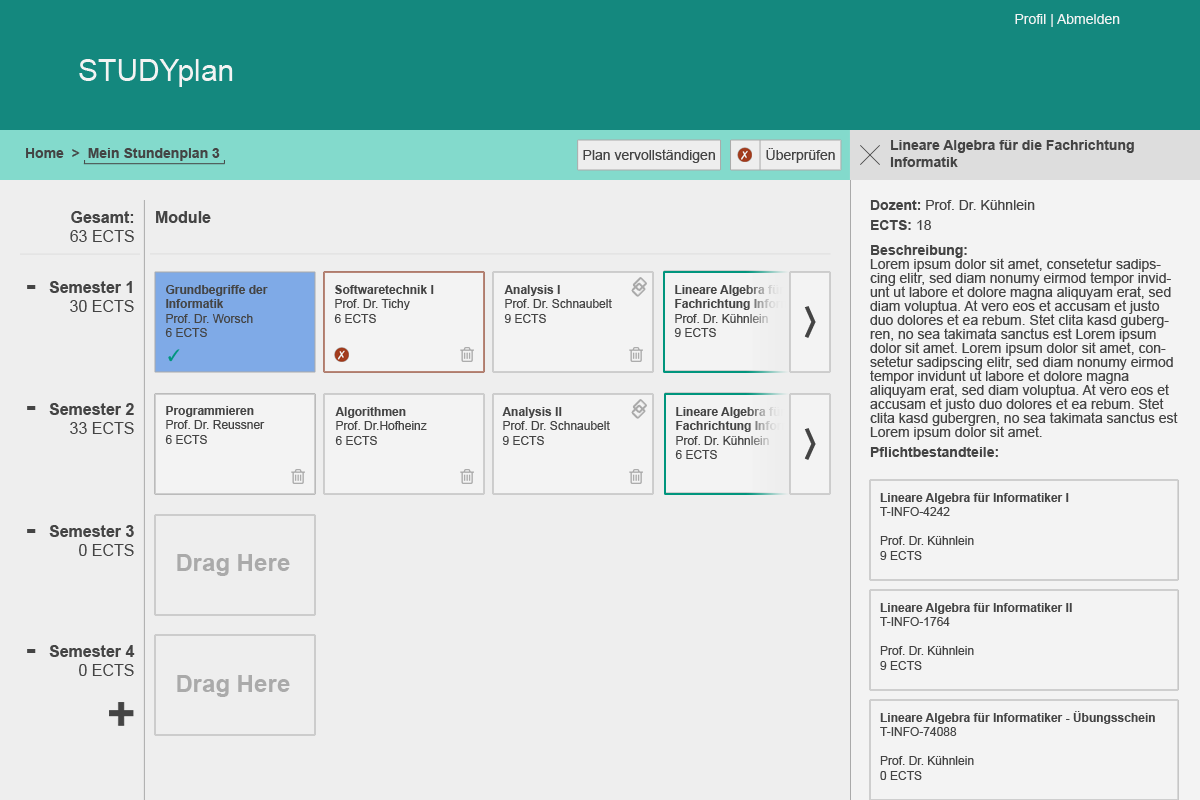
\includegraphics[width=0.9\textwidth]{../GUI/ergebnisse/verifizierung-2.png}
\end{figure}
\begin{figure}
	\caption{Profilansicht}
	\label{fig:gui-profil-1}
	\centering
	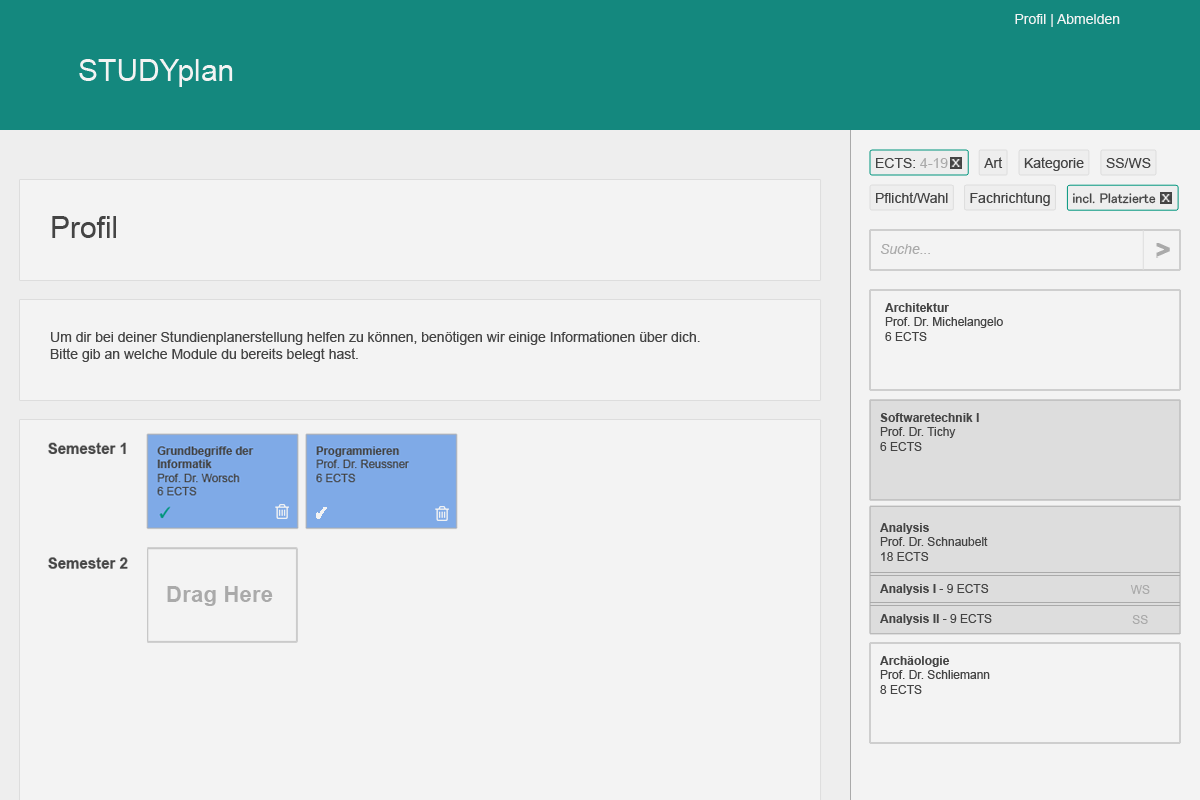
\includegraphics[width=0.9\textwidth]{../GUI/ergebnisse/profil-1.png}
\end{figure}
\FloatBarrier